\documentclass[12pt]{article}

\usepackage[a4paper,margin=1in]{geometry}
\usepackage{amsmath,amssymb}
\usepackage{newtxtext,newtxmath} % Times-style font
\usepackage{fancyhdr}
\usepackage{listings}
\usepackage{graphicx}
\usepackage{float}
\usepackage{algorithm}
\usepackage{algpseudocode}
\usepackage{xcolor}
\usepackage{booktabs}
\usepackage{array}

\setlength{\textfloatsep}{10pt}
\setlength{\floatsep}{10pt}

\setlength{\parindent}{0pt}
\setlength{\parskip}{5pt}

% Keep entire document at 12 pt
\AtBeginDocument{
    \fontsize{12pt}{14pt}\selectfont
}

\lstdefinestyle{code}{
    language=Python,
    basicstyle=\ttfamily\fontsize{10pt}{12pt}\selectfont,
    breaklines=true,
    breakatwhitespace=false,
    frame=single,
    numbers=left,
    numberstyle=\tiny\color{gray},
    keywordstyle=\color{blue},
    commentstyle=\color{gray},
    stringstyle=\color{green!50!black},
    columns=fullflexible,
    keepspaces=true,
    showstringspaces=false
}

\lstdefinestyle{output}{
    basicstyle=\ttfamily\fontsize{10pt}{12pt}\selectfont,
    breaklines=true,
    breakatwhitespace=false,
    frame=single,
    numbers=none,
    backgroundcolor=\color{gray!4},
    columns=fullflexible,
    keepspaces=true,
    showstringspaces=false
}

% ------------------------------------------------
% Header
% ------------------------------------------------

\pagestyle{fancy}
\fancyhf{}

\fancyhead[L]{Name: Kishan Sahu{\hspace{4cm}}}
\fancyhead[R]{Enrollment No.: P26DS017{\hspace{3.5cm}}}

\renewcommand{\headrulewidth}{0.4pt}
\setlength{\headheight}{15pt}

\begin{document}

% ------------------------------------------------
% TITLE
% ------------------------------------------------

\begin{center}
\textbf{Computer Science and Engineering Department, SVNIT, Surat}\\
\textbf{M.Tech. I -- Semester I}\\
\textbf{Design and Analysis of Algorithm (CSDS103)}\\
\textbf{Lab Assignment 4}\\
\textbf{Divide and Conquer}
\end{center}

\vspace{0.3cm}

\section{Introduction to Divide and Conquer}

The \textbf{Divide and Conquer} paradigm is a fundamental algorithmic design technique based on multi-branched recursion. It breaks a complex problem into smaller, independent subproblems of the same type, solves them recursively, and subsequently combines their individual solutions to construct the solution to the original problem. The paradigm adheres to three canonical phases:
\begin{enumerate}
    \item \textbf{Divide:} Partition the input problem into two or more disjoint subproblems of smaller size.
    \item \textbf{Conquer:} Solve the subproblems recursively. If the subproblem size is sufficiently small (the base case), solve it directly without further subdivision.
    \item \textbf{Combine:} Merge the solutions of the subproblems into a unified global solution.
\end{enumerate}

In this laboratory assignment, we analyze and implement two representative applications of the Divide and Conquer strategy:
\begin{itemize}
    \item \textbf{Problem 1 (Counting Inversions and Sorting Comparison):} Simultaneous sorting and inversion counting via an augmented Merge Sort in $O(n \log n)$ time, compared against an $O(n^2)$ Brute Force method, Quick Sort, and Insertion Sort.
    \item \textbf{Problem 2 (Fast Exponentiation):} Logarithmic computation of powers $a^n$ in $O(\log n)$ time via Divide and Conquer, contrasted against linear repeated multiplication and naive recursive branching.
\end{itemize}

\hrule
\vspace{0.3cm}

\section{Problem 1: Counting Inversions and Sorting Comparison}

\subsection{Problem Statement and Definitions}
Given an array $A = [a_1, a_2, \dots, a_n]$ of $n$ distinct elements, an \textbf{inversion} is defined as a pair of indices $(i, j)$ such that:
\begin{equation}
    i < j \quad \text{and} \quad A[i] > A[j]
\end{equation}
The inversion count measures how far an array is from being monotonically sorted. An array sorted in ascending order contains exactly $0$ inversions, whereas an array sorted in strictly descending order contains the maximum possible number of inversions:
\begin{equation}
    \binom{n}{2} = \frac{n(n-1)}{2} = \Theta(n^2)
\end{equation}
Counting inversions is central to various computational domains, including collaborative filtering algorithms, rank correlation coefficients (e.g., Kendall tau distance), and genomic distance metrics.

\subsection{Algorithmic Strategies}
\begin{enumerate}
    \item \textbf{Divide and Conquer Inversion Counter ($O(n \log n)$):}
    Modifies Merge Sort by dividing the array into two halves:
    \begin{itemize}
        \item Count inversions entirely contained within the left subarray ($inv_{\text{left}}$).
        \item Count inversions entirely contained within the right subarray ($inv_{\text{right}}$).
        \item Count split inversions where $i$ belongs to the left subarray and $j$ belongs to the right subarray ($inv_{\text{split}}$).
    \end{itemize}
    Because both halves are recursively sorted, when merging the two halves, if $A_{\text{left}}[i] > A_{\text{right}}[j]$, then every remaining element in $A_{\text{left}}$ from index $i$ to the end of the left subarray is strictly greater than $A_{\text{right}}[j]$. Hence, $\text{len}(A_{\text{left}}) - i$ split inversions are counted in $O(1)$ amortized steps per comparison.
    \item \textbf{Brute Force Inversion Counter ($O(n^2)$):}
    Examines every distinct pair of indices $(i, j)$ with $i < j$ via nested loops and increments a counter whenever $A[i] > A[j]$.
    \item \textbf{Baseline Sorting Benchmarks:}
    \begin{itemize}
        \item \textit{Quick Sort:} Standard partition-exchange sort with average-case time $\Theta(n \log n)$.
        \item \textit{Insertion Sort:} Incremental in-place sorting algorithm with average-case time $\Theta(n^2)$.
    \end{itemize}
\end{enumerate}

\subsection{Python Implementations}
The complete Python implementations from \texttt{DAA\_Lab4.ipynb} are listed below:

\begin{lstlisting}[style=code, caption={Problem 1 Algorithm Implementations}]
# 1. Divide and Conquer: Merge Sort and Count Inversions
def count_inversions_dc(arr):
    if len(arr) <= 1:
        return arr, 0
    mid = len(arr) // 2
    left, inv_left = count_inversions_dc(arr[:mid])
    right, inv_right = count_inversions_dc(arr[mid:])
    
    merged = []
    i = j = inv_split = 0
    while i < len(left) and j < len(right):
        if left[i] <= right[j]:
            merged.append(left[i])
            i += 1
        else:
            merged.append(right[j])
            inv_split += len(left) - i
            j += 1
    merged.extend(left[i:])
    merged.extend(right[j:])
    return merged, inv_left + inv_right + inv_split

# 2. Brute Force Inversion Counting
def count_inversions_bf(arr):
    inv = 0
    n = len(arr)
    for i in range(n):
        for j in range(i + 1, n):
            if arr[i] > arr[j]:
                inv += 1
    return inv

# 3. Baseline Sorting Algorithms for Comparison
def quick_sort(arr):
    if len(arr) <= 1:
        return arr
    pivot = arr[len(arr) // 2]
    left = [x for x in arr if x < pivot]
    mid = [x for x in arr if x == pivot]
    right = [x for x in arr if x > pivot]
    return quick_sort(left) + mid + quick_sort(right)

def insertion_sort(arr):
    a = arr.copy()
    for i in range(1, len(a)):
        key = a[i]
        j = i - 1
        while j >= 0 and a[j] > key:
            a[j + 1] = a[j]
            j -= 1
        a[j + 1] = key
    return a
\end{lstlisting}

\subsection{Verification on Sample Input}
The correctness of the implementations was verified using the reverse-sorted sample array $[8, 4, 2, 1]$. Because the elements are in strictly descending order, the total number of inversions is $\binom{4}{2} = 6$.

\begin{lstlisting}[style=output, caption={Console Output for Sample Verification}]
Original Array: [8, 4, 2, 1]
Divide & Conquer: Sorted = [1, 2, 4, 8], Inversions = 6
Brute Force:      Inversions = 6
\end{lstlisting}

Both algorithms correctly identify 6 inversions, confirming implementation fidelity.

\subsection{Experimental Performance Benchmarking}
To empirically compare the scaling behavior, randomly generated integer arrays of sizes $n \in \{100, 200, 400, 800, 1600, 3200\}$ were tested. The execution times (measured in seconds using high-resolution monotonic clocks) are summarized in Table~\ref{tab:p1_timings}.

\begin{table}[H]
\centering
\caption{Problem 1: Empirical Execution Times Across Input Sizes (seconds)}
\label{tab:p1_timings}
\vspace{0.2cm}
\begin{tabular}{rcccc}
\toprule
\textbf{Input Size ($n$)} & \textbf{D\&C Inversions ($s$)} & \textbf{Brute Force ($s$)} & \textbf{Quick Sort ($s$)} & \textbf{Insertion Sort ($s$)} \\
\midrule
100  & 0.000289 & 0.000328 & 0.000144 & 0.000194 \\
200  & 0.000424 & 0.001013 & 0.000271 & 0.000912 \\
400  & 0.000876 & 0.004677 & 0.000545 & 0.003223 \\
800  & 0.002905 & 0.025146 & 0.001013 & 0.014090 \\
1600 & 0.004140 & 0.090939 & 0.002461 & 0.057929 \\
3200 & 0.008791 & 0.405262 & 0.010584 & 0.545639 \\
\bottomrule
\end{tabular}
\end{table}

\begin{figure}[H]
\centering
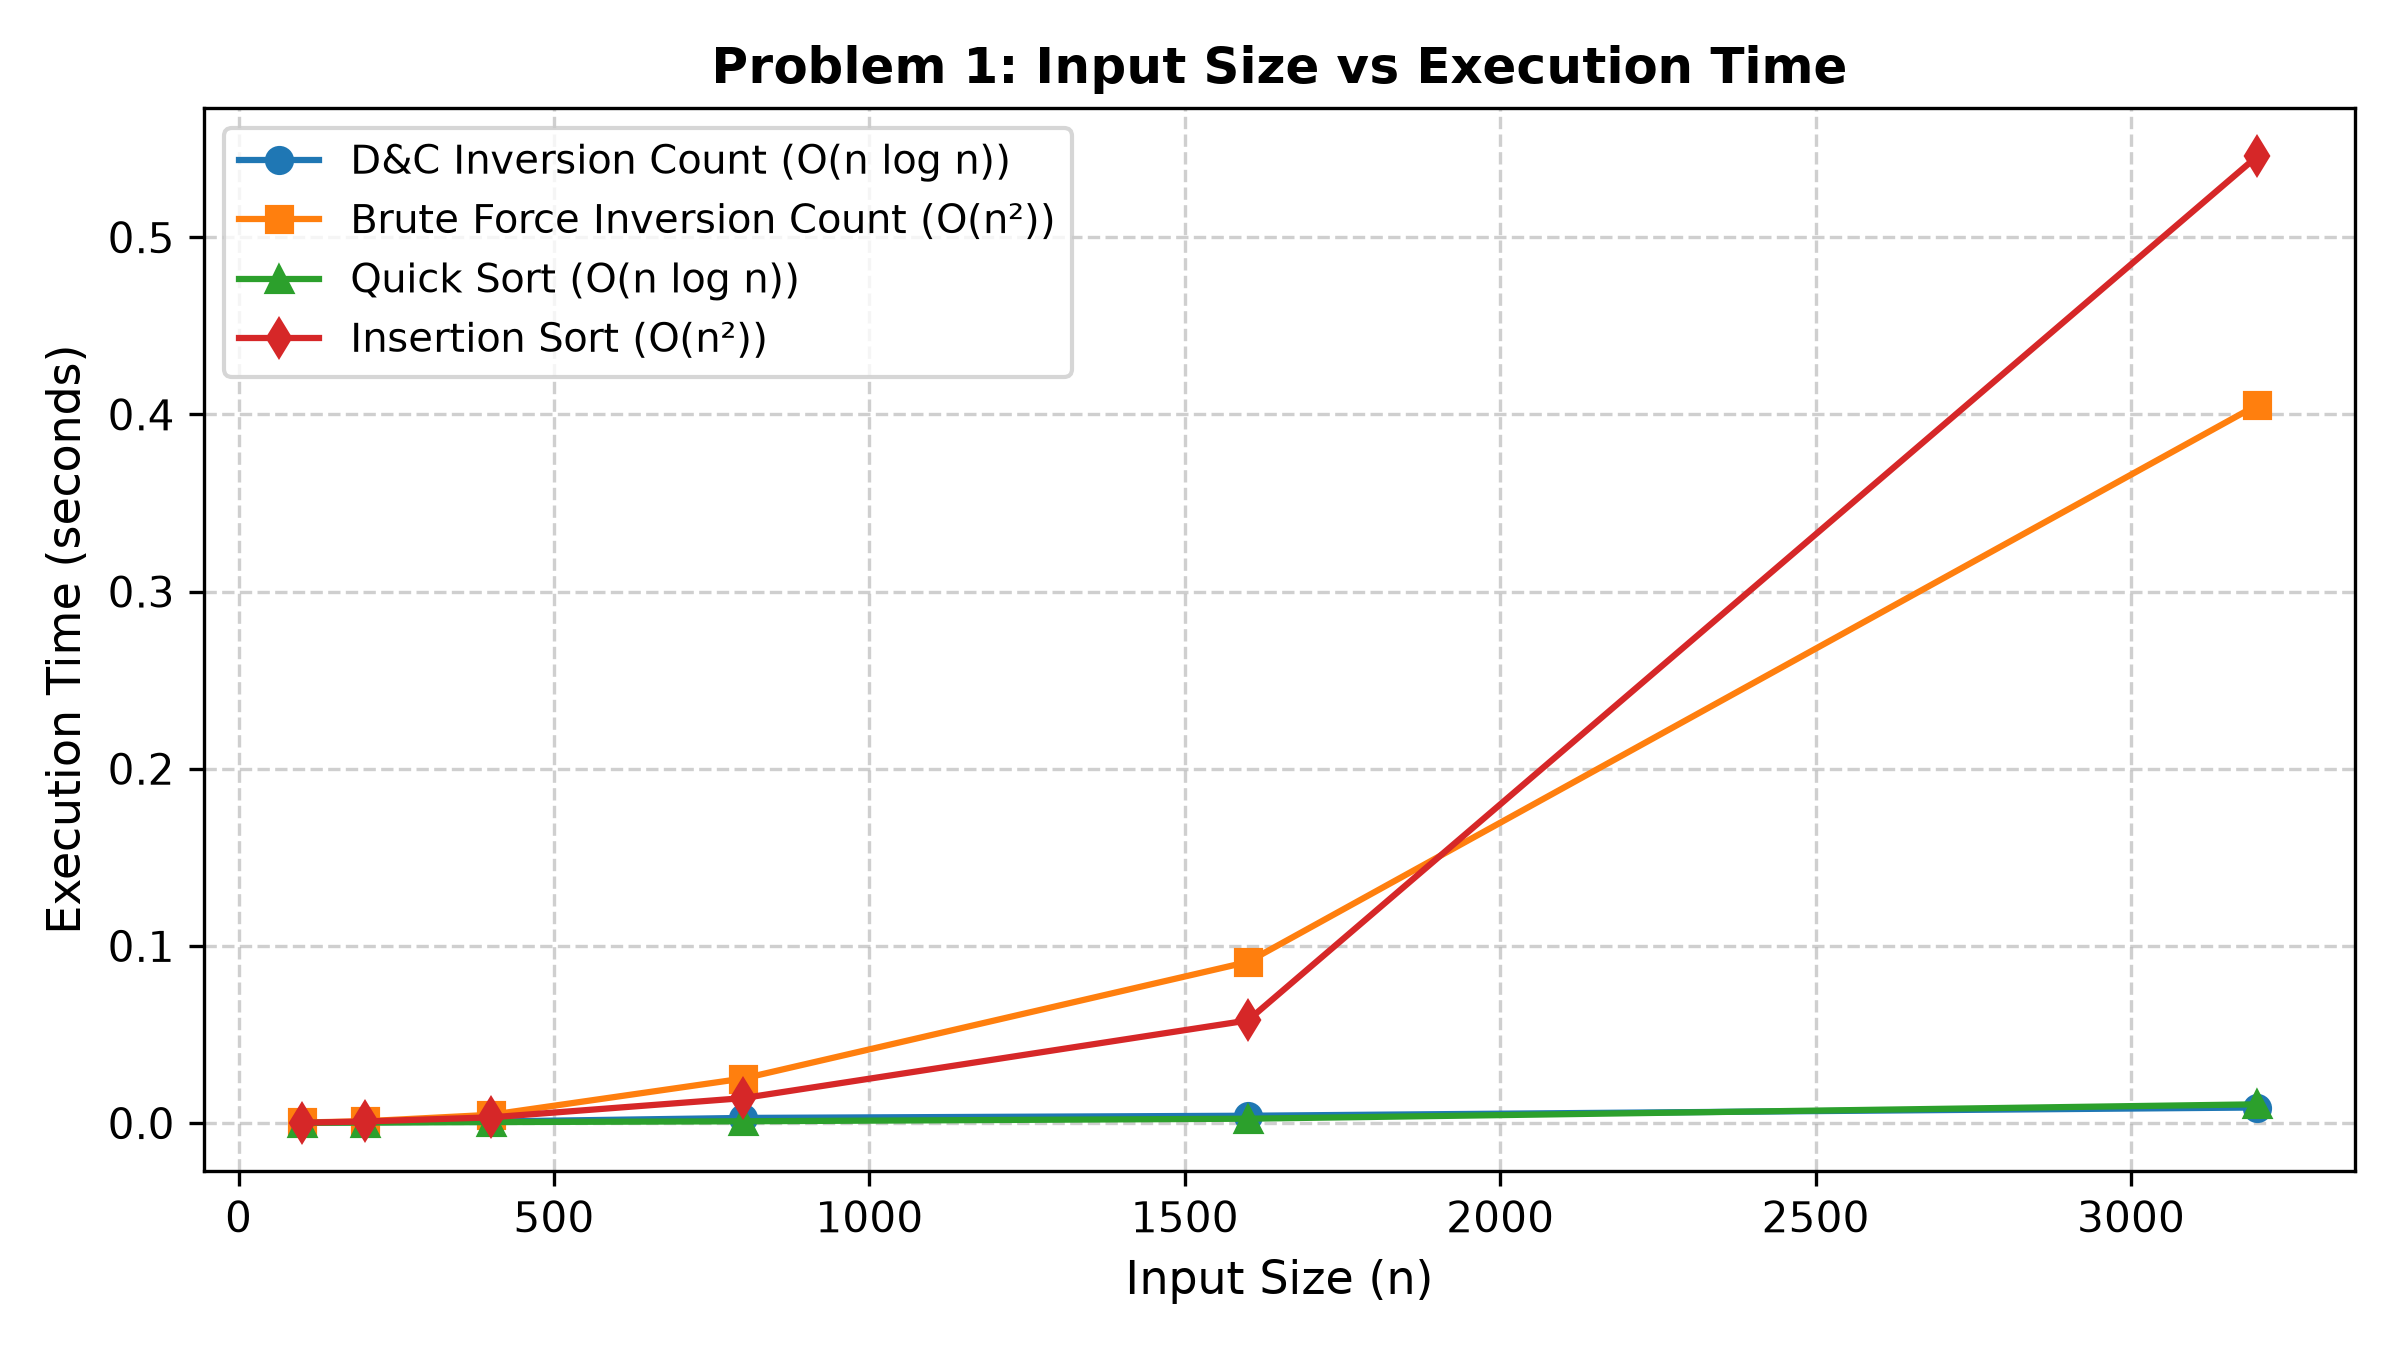
\includegraphics[width=0.88\linewidth]{figures/p1_inversion_benchmark.png}
\caption{Problem 1: Input Size ($n$) vs Execution Time (seconds) comparing Divide \& Conquer, Brute Force, Quick Sort, and Insertion Sort.}
\label{fig:p1_plot}
\end{figure}

\subsection{Theoretical Complexity and Experimental Analysis}
\begin{enumerate}
    \item \textbf{Divide and Conquer Complexity:}
    \begin{itemize}
        \item \textbf{Recurrence Relation:}
        \begin{equation}
            T(n) = 2T\left(\frac{n}{2}\right) + \Theta(n)
        \end{equation}
        where $2T(n/2)$ accounts for the two recursive subproblem invocations and $\Theta(n)$ represents the linear merging step where split inversions are tabulated.
        \item \textbf{Master Theorem Analysis:}
        For $T(n) = aT(n/b) + f(n)$ with $a = 2$, $b = 2$, and $f(n) = \Theta(n^d)$ with $d = 1$:
        \begin{equation}
            \log_b a = \log_2 2 = 1 = d
        \end{equation}
        By Case 2 of the Master Theorem:
        \begin{equation}
            T(n) = \Theta(n^{\log_b a} \log n) = \Theta(n \log n)
        \end{equation}
        \item \textbf{Auxiliary Space:}
        Requires $\Theta(n)$ auxiliary space to store temporary subarrays during the merge phase, along with $O(\log n)$ recursive call stack frames.
    \end{itemize}

    \item \textbf{Brute Force Complexity:}
    \begin{itemize}
        \item \textbf{Time Complexity:} The total number of pairwise comparisons is:
        \begin{equation}
            \sum_{i=0}^{n-2} \sum_{j=i+1}^{n-1} 1 = \sum_{i=1}^{n-1} (n - i) = \frac{n(n-1)}{2} = \Theta(n^2)
        \end{equation}
        Each comparison involves an $O(1)$ inequality check. Thus, time complexity is $\Theta(n^2)$.
        \item \textbf{Auxiliary Space:} Uses strictly $\Theta(1)$ auxiliary space as it performs pairwise scans in-place.
    \end{itemize}

    \item \textbf{Comparison with Baseline Sorting Algorithms:}
    \begin{itemize}
        \item \textit{Quick Sort:} Average time complexity $\Theta(n \log n)$, auxiliary space $O(\log n)$ recursion stack.
        \item \textit{Insertion Sort:} Average/Worst-case time complexity $\Theta(n^2)$, auxiliary space $O(1)$ in-place.
    \end{itemize}

    \item \textbf{Experimental vs. Theoretical Correspondence:}
    As illustrated in Figure~\ref{fig:p1_plot}, the quadratic curves for Brute Force Inversion Counting and Insertion Sort grow steeply ($405.2\,\text{ms}$ and $545.6\,\text{ms}$ at $n=3200$). In stark contrast, Divide and Conquer Inversion Counting and Quick Sort maintain nearly linear trajectories ($8.8\,\text{ms}$ and $10.6\,\text{ms}$ at $n=3200$), proving that the $O(n \log n)$ divide-and-conquer strategy offers an order-of-magnitude practical speedup for large datasets.
\end{enumerate}

\newpage

\section{Problem 2: Fast Exponentiation}

\subsection{Problem Statement and Definitions}
The exponentiation problem requires evaluating $a^n$ for a base $a \in \mathbb{R}$ (or $\mathbb{Z}$) and a non-negative integer exponent $n \in \mathbb{Z}_{\ge 0}$. For large values of $n$, standard linear evaluation becomes prohibitively inefficient.

\subsection{Algorithmic Approaches}
\begin{enumerate}
    \item \textbf{Repeated Multiplication ($O(n)$):}
    Directly computes $a^n = \underbrace{a \times a \times \dots \times a}_{n \text{ times}}$ using an iterative loop executing $n$ sequential multiplications.
    \item \textbf{Naive Recursive Exponentiation ($O(n)$):}
    Implements the piecewise mathematical identity without caching subproblems:
    \begin{equation}
        a^n = \begin{cases}
            1 & \text{if } n = 0 \\
            a^{n/2} \times a^{n/2} & \text{if } n \text{ is even} \\
            a \times a^{n-1} & \text{if } n \text{ is odd}
        \end{cases}
    \end{equation}
    Because both branches of $a^{n/2}$ are evaluated independently without memoization, redundant recursive subproblems cause exponential branching in the recurrence tree.
    \item \textbf{Divide and Conquer Exponentiation ($O(\log n)$):}
    Evaluates the subproblem $\text{half} = a^{\lfloor n/2 \rfloor}$ exactly once and stores it in a temporary variable:
    \begin{equation}
        a^n = \begin{cases}
            1 & \text{if } n = 0 \\
            (\text{half})^2 & \text{if } n \text{ is even} \\
            a \times (\text{half})^2 & \text{if } n \text{ is odd}
        \end{cases}
    \end{equation}
    \item \textbf{Iterative Divide and Conquer (Binary Exponentiation):}
    Evaluates powers iteratively by expressing the exponent $n$ in binary form: $n = \sum_{k=0}^{\lfloor \log_2 n \rfloor} b_k 2^k$, eliminating recursive call stack overhead completely.
\end{enumerate}

\subsection{Python Implementations}

\begin{lstlisting}[style=code, caption={Problem 2 Exponentiation Implementations}]
# 1. Repeated Multiplication
def power_iterative(a, n):
    res = 1
    for _ in range(n):
        res *= a
    return res

# 2. Recursive Exponentiation (Naive Branching from PDF Relation)
def power_recursive_naive(a, n):
    if n == 0:
        return 1
    if n % 2 == 0:
        return power_recursive_naive(a, n // 2) * power_recursive_naive(a, n // 2)
    else:
        return a * power_recursive_naive(a, n - 1)

# 3. Divide and Conquer Exponentiation (Subproblem Reused)
def power_dc(a, n):
    if n == 0:
        return 1
    half = power_dc(a, n // 2)
    if n % 2 == 0:
        return half * half
    else:
        return a * half * half

# 4. Iterative Divide and Conquer (Binary Exponentiation)
def power_dc_iterative(a, n):
    res = 1
    base = a
    while n > 0:
        if n % 2 == 1:
            res *= base
        base *= base
        n //= 2
    return res
\end{lstlisting}

\subsection{Verification on Sample Input}
The functions were verified for $a = 2, n = 10$, where the exact analytical result is $2^{10} = 1024$.

\begin{lstlisting}[style=output, caption={Console Output for Exponentiation Verification}]
Computing 2^10:
Repeated Multiplication : 1024
Naive Recursive         : 1024
Divide and Conquer      : 1024
Iterative D&C           : 1024
\end{lstlisting}

All four implementations produce the identical and correct output of 1024.

\subsection{Experimental Performance Benchmarking}
To assess empirical runtimes, the three principal algorithms were benchmarked for base $a = 2$ and exponents $n \in \{50, 100, 150, 200, 250, 300, 400, 500\}$. Each test was averaged over 100 iterations. Table~\ref{tab:p2_timings} presents the recorded runtimes.

\begin{table}[H]
\centering
\caption{Problem 2: Average Execution Times Across Exponents ($a = 2$)}
\label{tab:p2_timings}
\vspace{0.2cm}
\begin{tabular}{rccc}
\toprule
\textbf{Exponent ($n$)} & \textbf{Repeated Mult ($s$)} & \textbf{Naive Recursive ($s$)} & \textbf{Divide \& Conquer ($s$)} \\
\midrule
50  & $2.86 \times 10^{-6}$ & $1.16 \times 10^{-5}$ & $0.97 \times 10^{-6}$ \\
100 & $5.25 \times 10^{-6}$ & $2.09 \times 10^{-5}$ & $1.43 \times 10^{-6}$ \\
150 & $1.39 \times 10^{-5}$ & $4.48 \times 10^{-5}$ & $1.73 \times 10^{-6}$ \\
200 & $1.29 \times 10^{-5}$ & $4.41 \times 10^{-5}$ & $1.51 \times 10^{-6}$ \\
250 & $1.87 \times 10^{-5}$ & $5.97 \times 10^{-5}$ & $1.60 \times 10^{-6}$ \\
300 & $2.23 \times 10^{-5}$ & $7.93 \times 10^{-5}$ & $1.71 \times 10^{-6}$ \\
400 & $3.88 \times 10^{-5}$ & $9.49 \times 10^{-5}$ & $1.40 \times 10^{-6}$ \\
500 & $3.68 \times 10^{-5}$ & $1.08 \times 10^{-4}$ & $1.86 \times 10^{-6}$ \\
\bottomrule
\end{tabular}
\end{table}

\begin{figure}[H]
\centering
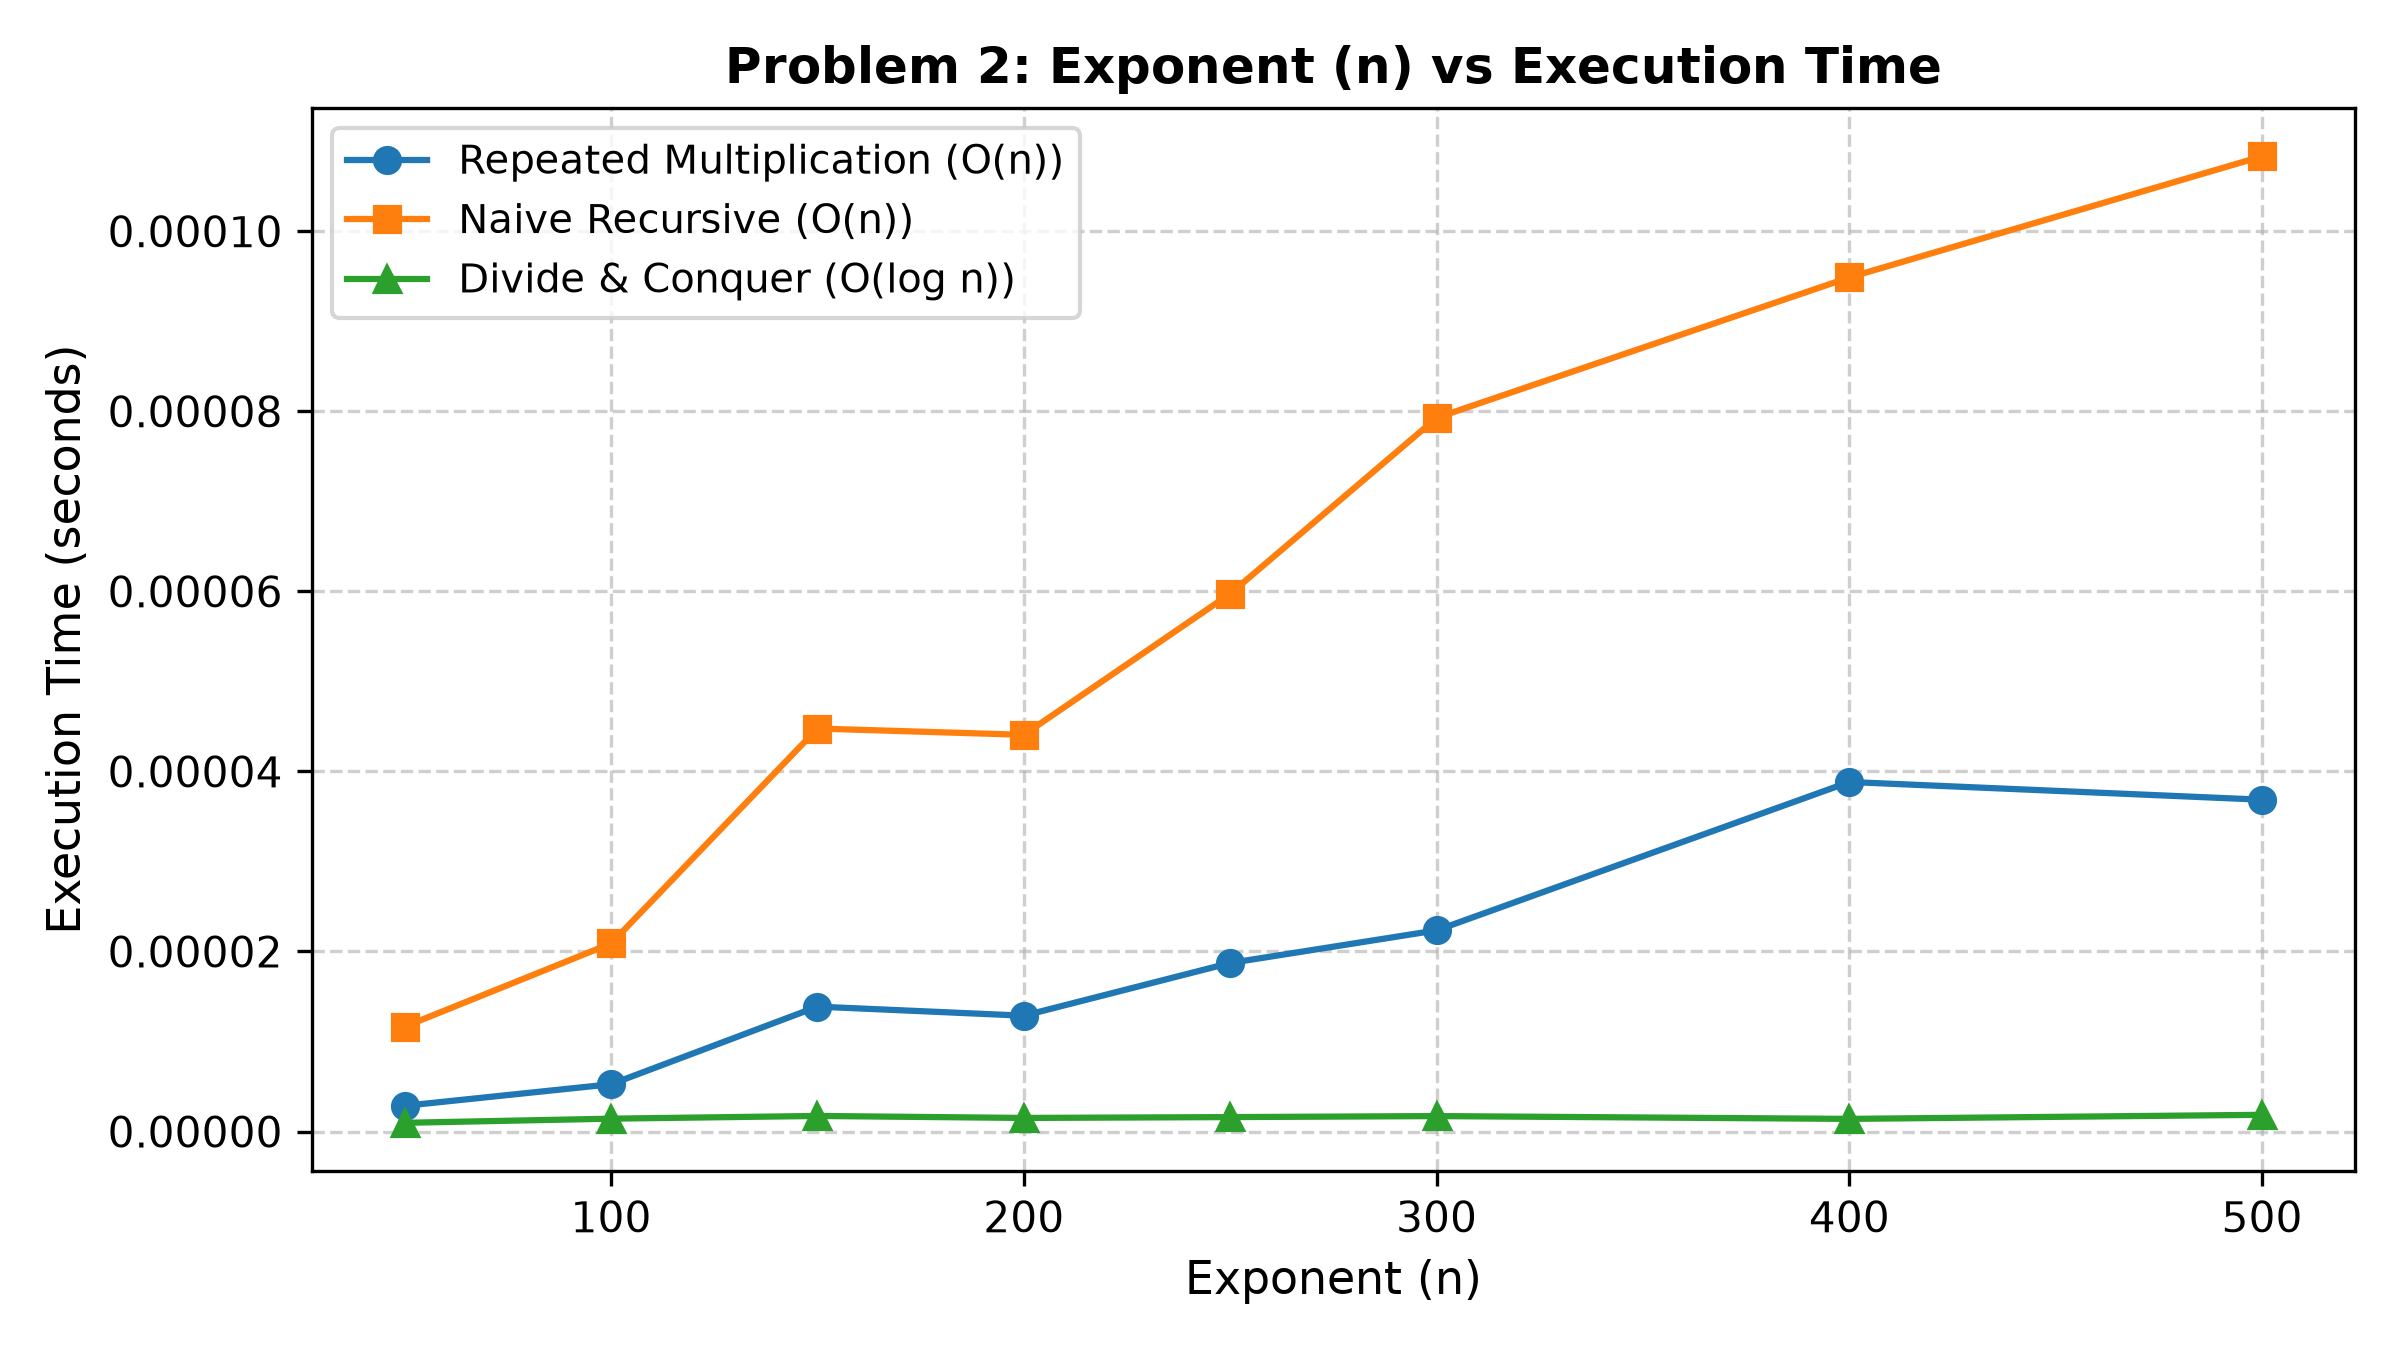
\includegraphics[width=0.88\linewidth]{figures/p2_exponentiation_benchmark.png}
\caption{Problem 2: Exponent ($n$) vs Execution Time (seconds) comparing Repeated Multiplication, Naive Recursive, and Divide \& Conquer.}
\label{fig:p2_plot}
\end{figure}

\subsection{Theoretical Analysis and Lab Questions}

\subsubsection{Question 1: Recurrence Relation for Divide and Conquer}
The Divide and Conquer algorithm computes $a^{\lfloor n/2 \rfloor}$ once and performs at most two multiplications (squaring $\text{half} \times \text{half}$, and multiplying by $a$ if $n$ is odd):
\begin{equation}
    T(n) = T\left(\left\lfloor \frac{n}{2} \right\rfloor\right) + \Theta(1)
\end{equation}
Using the Master Theorem $T(n) = aT(n/b) + f(n)$:
\begin{itemize}
    \item $a = 1$ (one subproblem solved recursively)
    \item $b = 2$ (subproblem size halved)
    \item $f(n) = \Theta(1) = \Theta(n^0) \implies d = 0$
\end{itemize}
Evaluating the exponent ratio:
\begin{equation}
    \log_b a = \log_2 1 = 0 = d
\end{equation}
Since $\log_b a = d$, by Case 2 of the Master Theorem:
\begin{equation}
    T(n) = \Theta(n^d \log n) = \Theta(\log n)
\end{equation}
The algorithm executes in strictly logarithmic time with respect to the exponent $n$.

\subsubsection{Question 2: Time and Auxiliary Space Complexity Summary}
Table~\ref{tab:comp_p2} summarizes the computational complexities of all three approaches:

\begin{table}[H]
\centering
\caption{Complexity Summary for Exponentiation Methods}
\label{tab:comp_p2}
\vspace{0.2cm}
\begin{tabular}{lcc}
\toprule
\textbf{Approach} & \textbf{Time Complexity} & \textbf{Auxiliary Space Complexity} \\
\midrule
Repeated Multiplication & $\Theta(n)$ & $\Theta(1)$ \\
Naive Recursive Exponentiation & $\Theta(n)$ & $\Theta(\log n)$ stack frames \\
Divide and Conquer Exponentiation & $\Theta(\log n)$ & $\Theta(\log n)$ stack frames \\
Iterative Divide and Conquer & $\Theta(\log n)$ & $\Theta(1)$ \\
\bottomrule
\end{tabular}
\end{table}

\subsubsection{Question 3: Effect of Repeatedly Computing Subproblems in the Naive Approach}
In the naive recursive definition:
\begin{equation*}
    \texttt{power\_recursive\_naive}(a, n//2) * \texttt{power\_recursive\_naive}(a, n//2)
\end{equation*}
both invocations evaluate the exact same expression independently. 
\begin{itemize}
    \item For an even exponent $n$, the recurrence is $T(n) = 2T(n/2) + O(1)$. By the Master Theorem ($a=2, b=2, d=0 \implies \log_2 2 = 1 > 0$), $T(n) = \Theta(n)$.
    \item The total number of recursive function calls grows linearly with $n$ (approximately $2n$ total invocations) rather than logarithmically.
    \item The Divide and Conquer algorithm caches the subproblem result in variable \texttt{half}, resolving the recurrence to $T(n) = T(n/2) + O(1)$, reducing the call tree depth to exactly $\lfloor \log_2 n \rfloor$ steps.
\end{itemize}

\subsubsection{Question 4: Why Reducing Multiplications Drastically Affects Execution Time for Large $n$}
When $n$ is very large, the number of bits in the result $a^n$ becomes enormous. Specifically, the bit length $b$ of $a^n$ is:
\begin{equation}
    b \approx \log_2(a^n) = n \log_2 a
\end{equation}
In real-world computer systems (such as Python's arbitrary-precision integers), multiplying two large $b$-bit numbers is \textbf{not} an $O(1)$ hardware instruction. Large integer multiplication takes super-linear bit complexity:
\begin{itemize}
    \item Karatsuba algorithm: $O(b^{\log_2 3}) \approx O(b^{1.585})$
    \item FFT-based multiplication: $O(b \log b \log \log b)$
\end{itemize}
In repeated multiplication, performing $n$ multiplications on growing integers requires accumulating bit-level overhead at every step, yielding an overall bit complexity of $O(n^2 \log^2 a)$. In contrast, Divide and Conquer performs only $\approx \log_2 n$ multiplications. The overwhelming majority of these multiplications occur on smaller intermediate bit lengths, achieving dramatic algorithmic acceleration.

\subsubsection{Question 5: Iterative Divide and Conquer and Auxiliary Space Elimination}
The recursive Divide and Conquer implementation requires $\lfloor \log_2 n \rfloor + 1$ stack frames, leading to $\Theta(\log n)$ auxiliary space. An iterative formulation (binary exponentiation) is implemented as:

\begin{lstlisting}[style=code, caption={Iterative Binary Exponentiation}]
def power_dc_iterative(a, n):
    res = 1
    base = a
    while n > 0:
        if n % 2 == 1:
            res *= base
        base *= base
        n //= 2
    return res
\end{lstlisting}

\textbf{Auxiliary Space Impact:}
\begin{itemize}
    \item The iterative approach uses only two local scalar variables (\texttt{res} and \texttt{base}) and avoids recursion entirely.
    \item Auxiliary memory consumption is reduced from $\Theta(\log n)$ stack frames to strictly \textbf{$\Theta(1)$ auxiliary space}.
\end{itemize}

\subsubsection{Question 6: Paradigm Comparison: Problem 1 vs Problem 2}
Both problems exploit the Divide and Conquer framework, but they exhibit distinct structural characteristics across the three phases:

\begin{table}[H]
\centering
\caption{Paradigm Comparison: Problem 1 vs Problem 2}
\label{tab:paradigm_comp}
\vspace{0.2cm}
\begin{tabular}{p{2.2cm}p{6.3cm}p{6.3cm}}
\toprule
\textbf{Phase} & \textbf{Problem 1: Inversion Counting} & \textbf{Problem 2: Fast Exponentiation} \\
\midrule
\textbf{Divide} & Partitions array into 2 halves of size $n/2$. & Reduces exponent $n$ into a single subproblem of size $\lfloor n/2 \rfloor$. \\
\addlinespace
\textbf{Conquer} & Recursively solves \textbf{both} subproblems ($2T(n/2)$). & Recursively solves only \textbf{one} subproblem ($1T(n/2)$). \\
\addlinespace
\textbf{Combine} & Merges the two sorted halves in linear time $\Theta(n)$ while counting split inversions. & Combines in $\Theta(1)$ time by squaring \texttt{half} (and multiplying by $a$ if $n$ is odd). \\
\addlinespace
\textbf{Overall Time} & $\Theta(n \log n)$ via Master Theorem Case 2 ($a=2, b=2, d=1$). & $\Theta(\log n)$ via Master Theorem Case 2 ($a=1, b=2, d=0$). \\
\bottomrule
\end{tabular}
\end{table}

\subsubsection{Question 7: Theoretical Complexity vs. Experimentally Observed Wall-Clock Time}
There is an inherent discrepancy between asymptotic theoretical complexity and experimental execution time:
\begin{enumerate}
    \item \textbf{Theoretical Complexity ($O$, $\Theta$, $\Omega$):} Focuses on asymptotic rates of operation growth as input size approaches infinity ($n \to \infty$). It abstracts away architecture-dependent constants, CPU pipelining, and system overhead.
    \item \textbf{Experimental Wall-Clock Time:} Measures physical elapsed time on actual hardware. It is influenced by:
    \begin{itemize}
        \item \textit{Constant factors:} Function call overhead in interpreted languages like Python (byte-code interpretation, dynamic typing).
        \item \textit{Memory hierarchy:} CPU L1/L2/L3 cache misses and RAM bandwidth during array allocation in merge sort.
        \item \textit{Operating system scheduling:} Context switching, timer tick resolution, and CPU frequency throttling (Turbo Boost / thermal throttling).
    \end{itemize}
\end{enumerate}
Despite these physical hardware variances, the empirical curves in Figures~\ref{fig:p1_plot} and~\ref{fig:p2_plot} closely corroborate the asymptotic orders of growth ($O(n^2)$ vs $O(n \log n)$ in Problem 1; $O(n)$ vs $O(\log n)$ in Problem 2).

\hrule
\vspace{0.3cm}

\section{Conclusion}
In this laboratory assignment, the Divide and Conquer paradigm was implemented, validated, and evaluated on two fundamental problems. For inversion counting, augmentations to Merge Sort reduced the runtime from $\Theta(n^2)$ to $\Theta(n \log n)$. For exponentiation, evaluating subproblems once reduced multiplications from $\Theta(n)$ to $\Theta(\log n)$, with binary exponentiation achieving optimal $\Theta(1)$ auxiliary space. The theoretical derivations via the Master Theorem were corroborated by empirical timing benchmarks.

\end{document}
